% !TEX root = ../../I4PRJ, Grp3 - Dokumentation.tex
I dette afsnit beskrives design og implementering af applikationslaget. Applikationslaget er det lag af software i det samlede distribuerede system, som installeres eller afvikles hos brugeren. Applikationslaget er designet til at være platformuafhængigt, jf. systemets arkitektur. Derved er lagets model- og præsentationslag designet til at være portabelt, hvorimod view-laget er platformspecifikt. På figur~\ref{fig:application_layer} ses det overordnede lagdiagram for applikationslagets design.

\begin{figure}
	\centering
	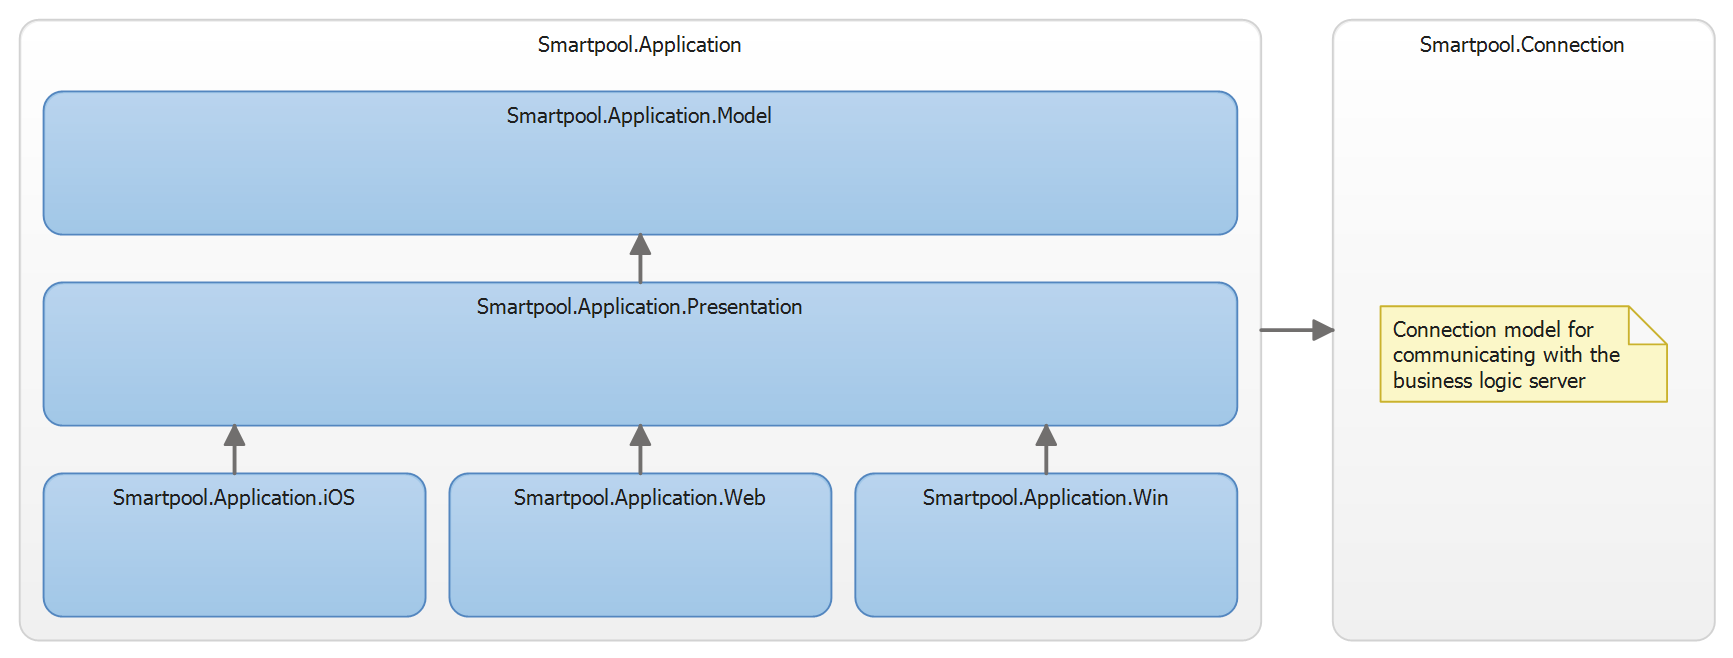
\includegraphics[width=1.0\linewidth]{figs/design/application_layer}
	\caption{Lagdiagram applikationslagets softwarepakker}
	\label{fig:application_layer}
\end{figure}

Af diagrammet fremgår det, at applikationslaget er opdelt i flere lag som følge af model-view-presenter arkitekturen, beskrevet i afsnittet arkitektur. En del af applikationslagets model findes i en separat pakke under navnet Smartpool.Connection. Denne pakke indeholder model-klasser til kommunikation mellem klient-applikationerne og Smartpools businesss-logic server.

Som følge af multi-lag arkitekturen kunne applikationslaget samt de platform-specifikke view-implementeringer designes, uafhængigt af hinanden, så længe interfaces blev specificeret undervejs i processen. Sammenkobling og protokolspecificering mellem de forskellige lag i applikationen er et resultat af interface specificeringen. Et eksempel på dette er rækken af view/presenter interfaces beskrevet i underafsnittet om design af applikationens præsentationslag.

Den overordnede ide omkring designet af model-view-presenter er adskillelse af lagene. View kalder presenter, som kan hente data fra model. Opstarts- og et interaktionsscenarie eksemplificeres på sekvensdiagrammet på figur~\ref{fig:application_sd}.

\begin{figure}
	\centering
	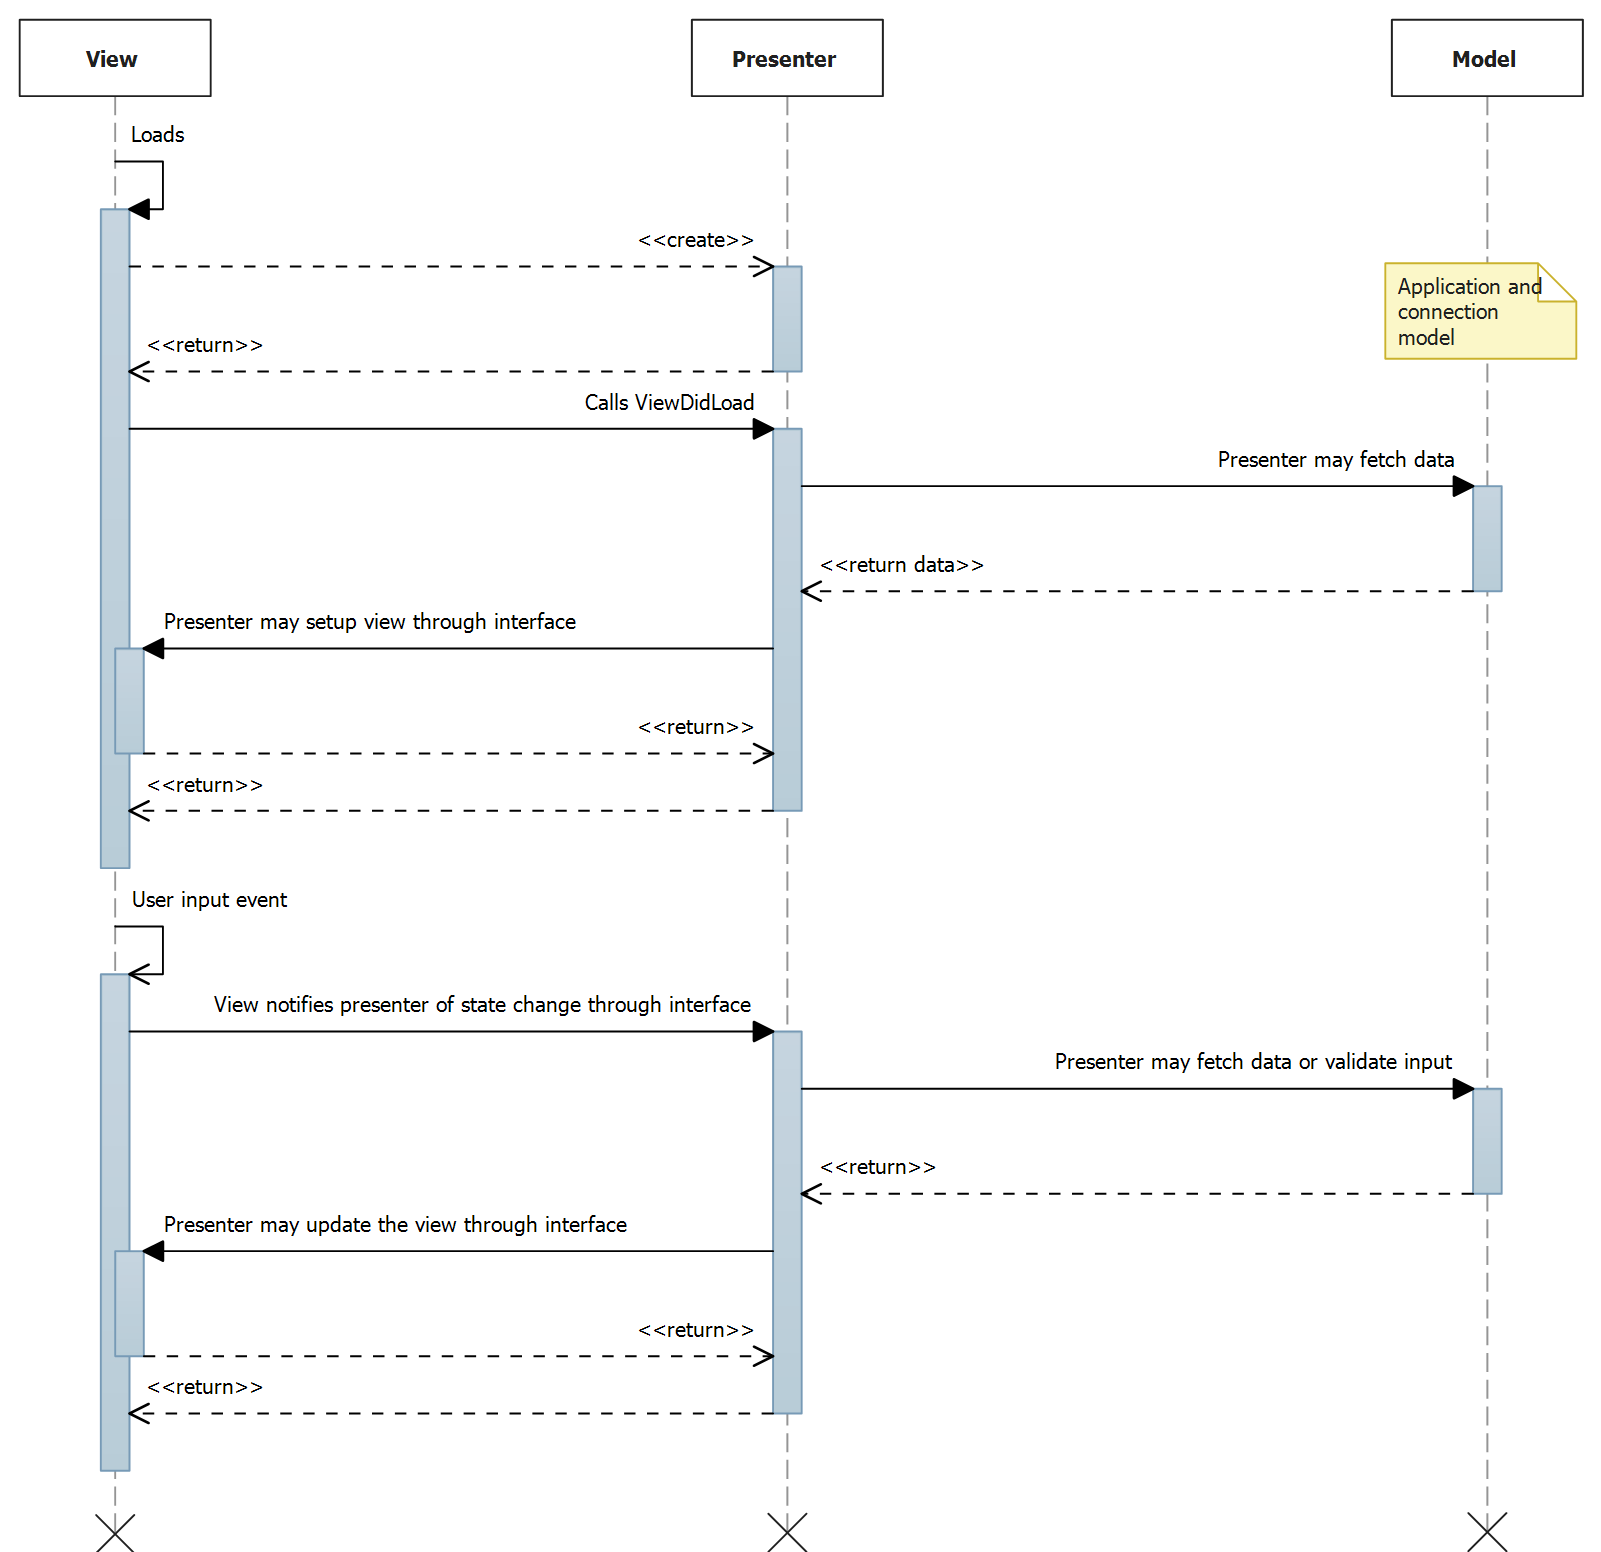
\includegraphics[width=1.0\linewidth]{figs/design/application_sd}
	\caption{Sekvensdiagram for det generelle interaktionsmønster i applikationslaget}
	\label{fig:application_sd}
\end{figure}

Implementeringen af applikationslaget består i, at implementere lagets modelklasser, presenterklasser og platform-specifikke user interface programmer. 